\subsubsection{Holzplatte}
Die verschiedenen Bereiche der Teststation werden mittels  3 Schicht Holzplatten, die eine Stärke von 18mm haben, getrennt. Diese Platten haben die Vorteile, dass sie sehr formstabil und langlebig sind. Außerdem weisen sie dank drei Schichten Massivholz eine hohe Biegefestigkeit. Dankensweise wurden uns die Platten von der Firma Tschabrun Herman Gesellschaft m.b.H. gesponsert. Da die Grundfläche vom Gestell die Fläche von 78x78cm hat, wird aus optischen Gründen die Arbeitsfläche mit den Maßen von 82x82cm gewählt. So steht die Platte auf jeder Seite 2cm über das Alugestell. Damit die Platten in der mittleren und unteren Ebene bündig mit dem Gestell sind, haben diese ein Maß von 78x78cm. Bei diesen Platten müssen die Ecken ausgesägt werden, damit sie formschlüssig mit dem Gestell sind. Diese Aussparungen sind 4x4cm groß, genauso groß wie die Aluprofile. 
\vspace{5mm}
\begin{figure}[H]
    \centering
    \begin{subfigure}[b]{0.4\textwidth}
        \centering
        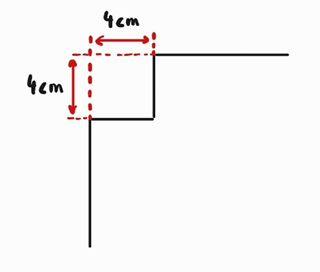
\includegraphics[width=\textwidth]{image/Bild1holzplatte.png}
        \caption{Aussparung Maße}
        \label{fig:bild1}
    \end{subfigure}
    \hfill
    \begin{subfigure}[b]{0.35\textwidth}
        \centering
        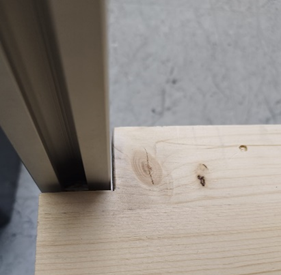
\includegraphics[width=\textwidth]{image/Bild2holzplatte.png}
        \caption{Aussparung umgesetzt}
        \label{fig:bild2}
    \end{subfigure}
    \caption{Aussparung}
    \label{fig:zwei_bilder}
\end{figure}
Damit die Wände befestigt werden können, werden in eine Holzplatte Nuten gefräst. So können die Platten nicht mehr verschoben werden und können fest verklebt werden. Die Nut ist 5mm tief und 8mm breit. Auf der Vorderseite, wird ein Stahlrahmen befestigt,  der auch in eine Nut eingelassen wird, diese Nut ist jedoch 4mm breit und 5mm tief. 
\vspace{5mm}
\begin{figure}[H]
    \centering
    \begin{subfigure}[b]{0.4\textwidth}
        \centering
        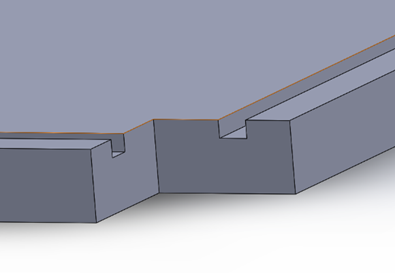
\includegraphics[width=\textwidth]{image/Bild1nut.png}
        
        \label{fig:bild1}
    \end{subfigure}
    \hfill
    \begin{subfigure}[b]{0.41\textwidth}
        \centering
        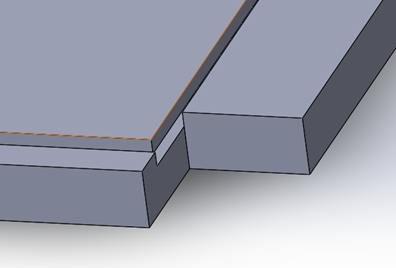
\includegraphics[width=\textwidth]{image/Bild2nut.png}
        
        \label{fig:bild2}
    \end{subfigure}
    \caption{Nut Vorderseite}
    \label{fig:zwei_bilder}
\end{figure}
Jede Holzplatte wird mit M8 Schrauben und Nutsteine angeschraubt. Dazu werden 8mm Löcher in die Holzplatten gebohrt und anschließen werden die die Löcher mit einem Senkbohrer gebohrt, dadurch können die Schrauben bündig mit der Platte verschraubt werden. 
\newpage